\begin{document}
%\tdplotsetmaincoords{0}{10}
\begin{tikzpicture}

  \def\r{0.5};
    \def\H{10};
    \pgfplotsset{ticks=none}
    \pgfplotsset{compat=1.12}
	\begin{axis}
		[
		view={-30}{0},
		scale=5,
		axis lines=center,
		axis on top,
		xlabel={$y$},
		ylabel={$x$},
		zlabel={$z$},
		domain=0:2,y domain=0:2,
		xmin=-1.5,
		xmax=1.5,
		ymin=-1.5,
		ymax=1.5,
		zmin=0.0,
		zmax=10.0,
		mesh/interior colormap=
		{blueblack}{color=(gray) color=(gray!50)},
		colormap=
		{blueblack}{color=(white) color=(white!50)},
		samples=10,
		samples y=40,
		z buffer=sort,
		]
				%draw the cylinder
		\addplot3 [surf]({\r*cos(deg(y))},{\r*sin(deg(y))},{x});
		
%\addplot3[red, ultra thick, domain=130:200, samples=20, samples y=1] ( {cos(x)*0.4+0.3}, {sin(x)*0.4-0.4}, {sqrt(1-((cos(x)*0.4+0.3))^2-((sin(x)*0.4-0.4))^2))} );
%\addplot3[blue, ultra thick, domain=0:360, samples=200, samples y=1] ( {0.5*cos(x)}, {0.5*sin(x)},{0.01*x} );
         \addplot3+[domain=0:2*pi,samples y=0]
            ({sin(deg(x))},
             {cos(deg(x))},
             {x});
	\end{axis}
\end{tikzpicture}
\end{document} 

tdplotsetmaincoords{60}{110}


\pgfplotsset{compat=1.12}
\begin{document}
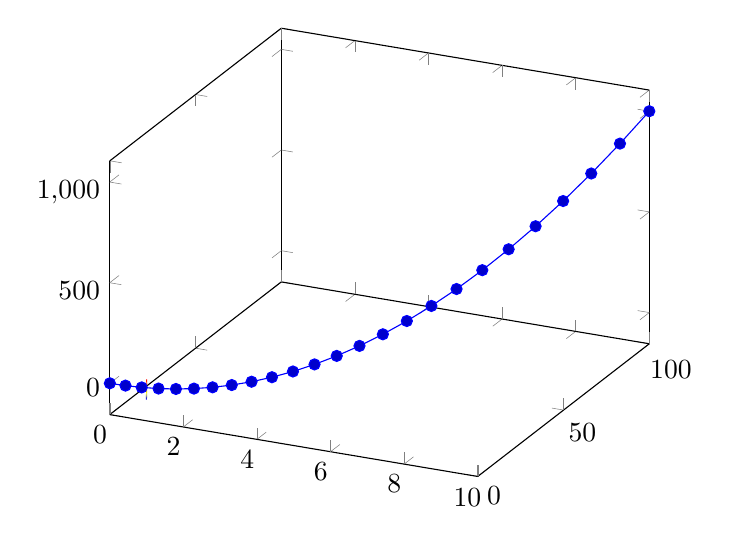
\begin{tikzpicture}
    \begin{axis}[samples y=0]
        \addplot3+[domain=0:10] (x,x^2,x^3);
        %draw the cylinder
	\addplot3 [surf]({cos(x)},{sin(x)},{10*x});
    \end{axis}
\end{tikzpicture}

\end{document}